\section{System Architecture}

\begin{frame}{System Architecture Overview}
  \begin{center}
    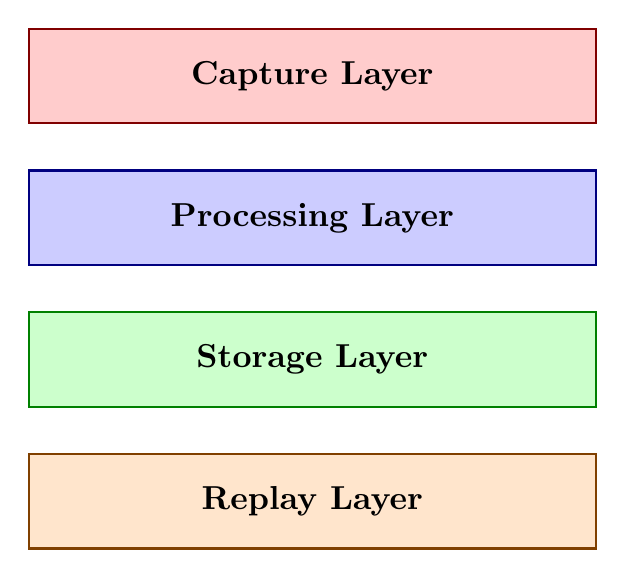
\begin{tikzpicture}[scale=1.2, every node/.style={scale=1.2}]
      % Capture Layer
      \draw[fill=red!20, draw=red!50!black, thick] (0,4.5) rectangle (6,5.5);
      \node at (3,5) {\textbf{Capture Layer}};

      % Processing Layer
      \draw[fill=blue!20, draw=blue!50!black, thick] (0,3) rectangle (6,4);
      \node at (3,3.5) {\textbf{Processing Layer}};

      % Storage Layer
      \draw[fill=green!20, draw=green!50!black, thick] (0,1.5) rectangle (6,2.5);
      \node at (3,2) {\textbf{Storage Layer}};

      % Replay Layer
      \draw[fill=orange!20, draw=orange!50!black, thick] (0,0) rectangle (6,1);
      \node at (3,0.5) {\textbf{Replay Layer}};
    \end{tikzpicture}
  \end{center}
\end{frame}

\begin{frame}{System Architecture - Core Components}
  \begin{block}{Core Components}
    \begin{itemize}
      \item \textbf{Capture Layer}
        \begin{itemize}
          \scriptsize
          \item AI Tool Plugins (Claude Code, Gemini, Copilot)
          \item Git Hook Integration
          \item CLI Monitoring Tool
        \end{itemize}

      \item \textbf{Storage Layer}
        \begin{itemize}
          \scriptsize
          \item Local: \texttt{.prompts/} directory in git repository
          \item Schema validation engine
          \item Git-based versioning
        \end{itemize}

      \item \textbf{Processing Layer}
        \begin{itemize}
          \scriptsize
          \item Prompt parser and validator
          \item Context extractor (dependencies, environment)
          \item Metadata enrichment (commit hash, file tracking)
        \end{itemize}

      \item \textbf{Replay Layer}
        \begin{itemize}
          \scriptsize
          \item Prompt reconstruction engine
          \item Cross-language translation adapter
          \item Validation framework
        \end{itemize}
    \end{itemize}
  \end{block}
\end{frame}

\begin{frame}{Data Flow Architecture - Capture \& Storage}
  \begin{block}{1. Capture Phase}
    \begin{itemize}
      \item Developer initiates AI session
      \item Plugin/CLI captures prompts in real-time
      \item Metadata extracted: timestamps, tool version, context
      \item Files tracked: generated, modified, deleted
    \end{itemize}
  \end{block}

  \begin{block}{2. Storage Phase}
    \begin{itemize}
      \item Prompts serialized to YAML/JSON
      \item Schema validation before commit
      \item Git commit linked to prompt file
      \item Hash-based deduplication
    \end{itemize}
  \end{block}
\end{frame}

\begin{frame}{Data Flow Architecture - Retrieval \& Replay}
  \begin{block}{3. Retrieval Phase}
    \begin{itemize}
      \item Search by keywords, tags, file paths
      \item Filter by AI tool, language, date range
      \item Dependency analysis for related prompts
    \end{itemize}
  \end{block}

  \begin{block}{4. Replay Phase}
    \begin{itemize}
      \item Load prompt history
      \item Adapt context to target environment
      \item Execute prompts against AI tool
      \item Validate output against original
    \end{itemize}
  \end{block}
\end{frame}

\begin{frame}{Integration Points - AI Tools}
  \begin{block}{MCP-Based Integration}
    \begin{itemize}
      \scriptsize
      \item \textbf{MCP Server}: Acts as middleware between AI tools and prompt storage
      \item \textbf{Protocol Standardization}: Unified interface for multiple AI tools
      \item \textbf{Tool Call Tracking}: Captures all tool invocations and results
      \item \textbf{Context Management}: Preserves conversation state and artifacts
      \item \textbf{Replay Support}: Re-executes captured prompts with full context
    \end{itemize}
  \end{block}

  \begin{block}{API-Based Integration}
    \begin{itemize}
      \scriptsize
      \item Direct integration via official APIs
      \item Claude API, Gemini API, OpenAI API
      \item Capture request/response pairs
      \item Preserve model parameters and settings
    \end{itemize}
  \end{block}

  \begin{block}{Plugin-Based Integration}
    \begin{itemize}
      \scriptsize
      \item Editor/IDE extensions (VS Code, JetBrains, Vim/Emacs)
    \end{itemize}
  \end{block}
\end{frame}

\begin{frame}{Integration Points - Version Control}
  \begin{block}{Git Integration}
    \begin{itemize}
      \item \textbf{Pre-commit Hook}: Validate prompt files before commit
      \item \textbf{Post-commit Hook}: Link prompts to commit hash
      \item \textbf{CI/CD}: Automated testing of prompt replay
      \item \textbf{.gitignore Patterns}: Exclude sensitive prompts
    \end{itemize}
  \end{block}

  \begin{block}{Benefits}
    \begin{itemize}
      \item Seamless integration with existing workflows
      \item Automatic prompt tracking
      \item Version history maintained with code
    \end{itemize}
  \end{block}
\end{frame}
